\section{Results and Discussion}
\label{sec:results}

This section presents the quantitative, computational, and qualitative results obtained across the LLFF benchmark. Table~\ref{tab:super_results} reports the global averages for reconstruction fidelity, training time, rendering throughput, and dynamic memory allocation across all evaluated regimes.

\begin{table}[!t]
\centering
\caption{Consolidated benchmark results on the LLFF dataset. Values represent global averages across valid test scenes. Training time corresponds to the best 500-step fine-tuning configuration for generalizable models (including test-view evaluation) and 30,000-step convergence for Per-Scene models ($N=10$). VRAM indicates peak dynamic memory allocated during inference.}
\label{tab:super_results}
\scriptsize
\setlength{\tabcolsep}{1.8pt}
\begin{tabular*}{\linewidth}{@{\extracolsep{\fill}}llcccccc@{\extracolsep{0pt}}}
\toprule
Model & Regime 
  & PSNR $\uparrow$ 
  & SSIM $\uparrow$ 
  & LPIPS $\downarrow$ 
  & Time $\downarrow$
  & FPS $\uparrow$ 
  & VRAM $\downarrow$ \\
\midrule
\multirow{2}{*}{PixelNeRF}
 & ZS  & 6.35  & 0.085 & 0.800 & $\sim$22 s   & 0.004 & 1.93 \\
 & FT  & 10.92 & 0.162 & 0.772 & 4 min 36 s   & 0.006 & 1.97 \\
\midrule
\multirow{2}{*}{GNT}
 & ZS  & 10.51 & 0.314 & 0.742 & \textbf{$\sim$9 s}    & 0.014 & 1.94 \\
 & FT  & 15.07 & 0.368 & 0.679 & 4 min 59 s   & 0.015 & 1.93 \\
\midrule
Instant-NGP
 & N=10   & 14.06 & 0.442 & 0.498 & 31 min 51 s  & 0.199 & 1.09 \\
\midrule
Nerfacto
 & N=10   & \textbf{27.11} & \textbf{0.875} & \textbf{0.171} & 8 min 57 s   & 0.388 & 1.43 \\
\midrule
Splatfacto
 & N=10   & 24.80 & 0.830 & 0.210 & 16 min 23 s  & \textbf{200.7} & \textbf{0.10} \\
\bottomrule
\end{tabular*}
\end{table}

\subsection{Visual Fidelity Across Paradigms}
Under $N=10$ input views, per-scene methods that incorporate spatial proposal sampling or explicit 3D primitives achieved the highest visual quality. Nerfacto obtained the best overall metrics at $27.11$ dB PSNR, $0.875$ SSIM, and $0.171$ LPIPS (Table~\ref{tab:super_results}), followed by Splatfacto (3DGS) with $24.80$ dB PSNR, $0.830$ SSIM, and $0.210$ LPIPS. Initializing anisotropic 3D Gaussians from sparse COLMAP point clouds preserved structural boundaries and high-frequency textures across test views. By comparison, Instant-NGP lacked sparse-view depth regularization and overfitted to the training rays, reaching $14.06$ dB PSNR.

For the generalizable architectures, direct Zero-Shot (ZS) inference was affected by domain shift and wide baselines between cameras. PixelNeRF obtained $6.35$ dB PSNR and $0.800$ LPIPS in zero-shot mode, whereas GNT reached $10.51$ dB PSNR and $0.314$ SSIM through its epipolar cross-attention mechanism. After fine-tuning on the target views, GNT improved to $15.07$ dB PSNR (and up to $17.46$ dB on \textit{fortress}), outperforming per-scene Instant-NGP ($14.06$ dB) in less training time ($4\text{ min }59\text{ s}$ vs.\ $31\text{ min }51\text{ s}$). Fine-tuning also raised PixelNeRF by $+4.57$ dB to $10.92$ dB PSNR under backbone adaptation, although its rendered views remained spatially blurred.

\subsection{Comparative Analysis of Fine-Tuning Strategies}
\label{sec:ft_results}

Table~\ref{tab:mixed_model_comparison} and Figure~\ref{fig:ft_efficiency_bars} summarize the multi-seed reconstruction metrics and execution times across the five fine-tuning strategies for PixelNeRF (5 valid scenes) and GNT (6 valid scenes). The results show opposite adaptation requirements between the convolutional and transformer-based architectures.

\begin{table}[!t]
\centering
\caption{Multi-seed evaluation of fine-tuning strategies on PixelNeRF (5 valid scenes) and GNT (6 valid scenes) across seeds $\{42, 123, 999\}$ at $500$ steps. CNN-based PixelNeRF achieved its highest PSNR under encoder adaptation (\textit{PFT-Backbone}), whereas transformer-based GNT performed best under epipolar decoder tuning (\textit{PFT-Decoder}) and low-rank adaptation (\textit{PEFT-LoRA}).}
\label{tab:mixed_model_comparison}
\scriptsize
\setlength{\tabcolsep}{2.5pt}
\begin{tabular*}{\linewidth}{@{\extracolsep{\fill}}llccccc@{\extracolsep{0pt}}}
\toprule
Model & Strategy & $\eta$ & $r$ & PSNR (dB) $\uparrow$ & SSIM $\uparrow$ & LPIPS $\downarrow$ \\
\midrule
\multirow{6}{*}{PixelNeRF}
 & Zero-Shot (ZS)   & N/A        & N/A    & 6.35 $\pm$ 0.05            & 0.085    & 0.800    \\
 & Full-FT          & $10^{-4}$  & N/A    & 9.03 $\pm$ 0.11            & 0.136    & 0.752    \\
 & PFT-Decoder      & $10^{-4}$  & N/A    & 10.58 $\pm$ 0.08           & \textbf{0.205} & 0.773    \\
 & PFT-Backbone     & $10^{-4}$  & N/A    & \textbf{10.92} $\pm$ 0.26  & 0.162    & 0.772    \\
 & BitFit           & $10^{-4}$  & N/A    & 10.79 $\pm$ 0.19           & 0.119    & 0.775    \\
 & PEFT-LoRA        & $10^{-3}$  & 4      & 8.59 $\pm$ 0.10            & 0.175    & \textbf{0.725} \\
\midrule
\multirow{6}{*}{GNT}
 & Zero-Shot (ZS)   & N/A        & N/A    & 10.51 $\pm$ 0.11           & 0.314    & 0.742    \\
 & Full-FT          & $10^{-3}$  & N/A    & 15.06 $\pm$ 0.03           & \textbf{0.369} & 0.681    \\
 & PFT-Decoder      & $10^{-3}$  & N/A    & \textbf{15.07} $\pm$ 0.03  & 0.368    & \textbf{0.679} \\
 & PFT-Backbone     & $10^{-4}$  & N/A    & 10.51 $\pm$ 0.11           & 0.314    & 0.742    \\
 & BitFit           & $10^{-3}$  & N/A    & 13.12 $\pm$ 0.05            & 0.358    & 0.742    \\
 & PEFT-LoRA        & $10^{-3}$  & 4      & 14.57 $\pm$ 0.07           & \textbf{0.369} & 0.706    \\
\bottomrule
\end{tabular*}
\end{table}

\begin{figure}[!t]
\centering
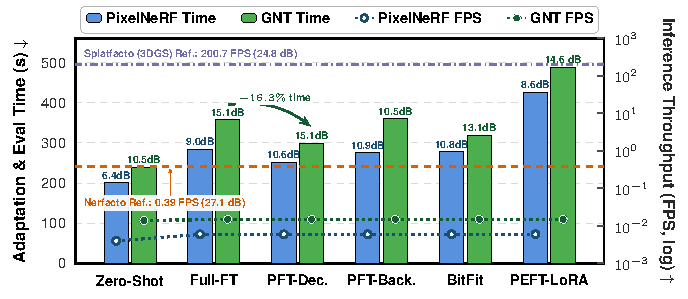
\includegraphics[width=\linewidth]{img/plot_ft_bars.pdf}
\vspace{-4pt}
\caption{Adaptation and evaluation time (bars, left axis, annotated with mean PSNR) and rendering throughput in FPS (markers, right log-axis) across fine-tuning strategies for PixelNeRF and GNT, compared against Nerfacto and Splatfacto (3DGS) reference lines. In GNT, \textit{PFT-Decoder} matched \textit{Full-FT} accuracy ($15.07$ dB) while reducing adaptation time by $16.3\%$ ($298.8\text{ s}$ vs.\ $357.1\text{ s}$). \textit{PEFT-LoRA} ($r=4$) required longer training time ($488.0\text{ s}$) due to adapter projections during backpropagation, but maintained native inference speed ($0.015$ FPS) after in-place weight merging.}
\label{fig:ft_efficiency_bars}
\end{figure}

In PixelNeRF, the highest PSNR was obtained when restricting gradient updates to the ResNet encoder (\textit{PFT-Backbone}, $10.92 \pm 0.26$ dB in $275.7\text{ s}$) or to additive biases (\textit{BitFit}, $10.79 \pm 0.19$ dB in $277.7\text{ s}$), both of which outperformed \textit{Full-FT} ($9.03 \pm 0.11$ dB in $284.8\text{ s}$). Because PixelNeRF projects 2D feature maps onto 3D rays, adjusting the convolutional filters to the target scene illumination improved color consistency, whereas updating all weights simultaneously destabilized the downstream MLP. Table~\ref{tab:mixed_model_comparison} also indicates a difference between pixel-level and perceptual metrics: \textit{PFT-Backbone} maximized PSNR through smooth color averaging, while \textit{PFT-Decoder} reached the highest structural similarity ($0.205$ SSIM in $252.0\text{ s}$) and \textit{PEFT-LoRA} ($r=4$) obtained the lowest perceptual error ($0.725$ LPIPS vs.\ $0.772$ for \textit{PFT-Backbone}) despite a lower PSNR ($8.59$ dB).

In GNT, the best reconstruction quality was achieved under \textit{PFT-Decoder} ($15.07 \pm 0.03$ dB PSNR and $0.679$ LPIPS), matching \textit{Full-FT} ($15.06 \pm 0.03$ dB) while avoiding backpropagation through the ViT encoder and reducing adaptation time from $357.1\text{ s}$ to $298.8\text{ s}$ (a $16.3\%$ reduction, Figure~\ref{fig:ft_efficiency_bars}). Freezing the pre-trained ViT encoder preserved its visual representations and concentrated weight updates within the epipolar cross-attention layers. In contrast, \textit{PFT-Backbone} produced no improvement over Zero-Shot ($10.51 \pm 0.11$ dB in $360.8\text{ s}$), showing that GNT adaptation depends on epipolar ray aggregation rather than shallow 2D patch projections. Parameter-efficient strategies also regularized GNT training: \textit{BitFit} reached $13.12 \pm 0.05$ dB ($+2.61$ dB over ZS in $319.0\text{ s}$) by updating $<0.15\%$ of the weights, and \textit{PEFT-LoRA} ($r=4$) reached $14.57 \pm 0.07$ dB and $0.369$ SSIM. Although evaluating the auxiliary \texttt{LoRALinear} branches during training increased execution time ($488.0\text{ s}$ in GNT and $426.4\text{ s}$ in PixelNeRF), merging $\Delta W = \frac{\alpha}{r}BA$ into $W_0$ before evaluation preserved the baseline rendering speed ($0.015$ and $0.006$ FPS).

\subsection{Computational Efficiency and Pareto Trade-offs}
Figures~\ref{fig:boxplot} and~\ref{fig:radar_chart} present the PSNR distribution across scenes and the five-axis trade-off profile across fidelity and hardware metrics. Generalizable models exhibited low inter-scene variance in Zero-Shot mode, which expanded after fine-tuning as the networks adapted to scene-specific geometry, whereas per-scene models showed wider variance driven by scene texture complexity.

\begin{figure}[!t]
\centering
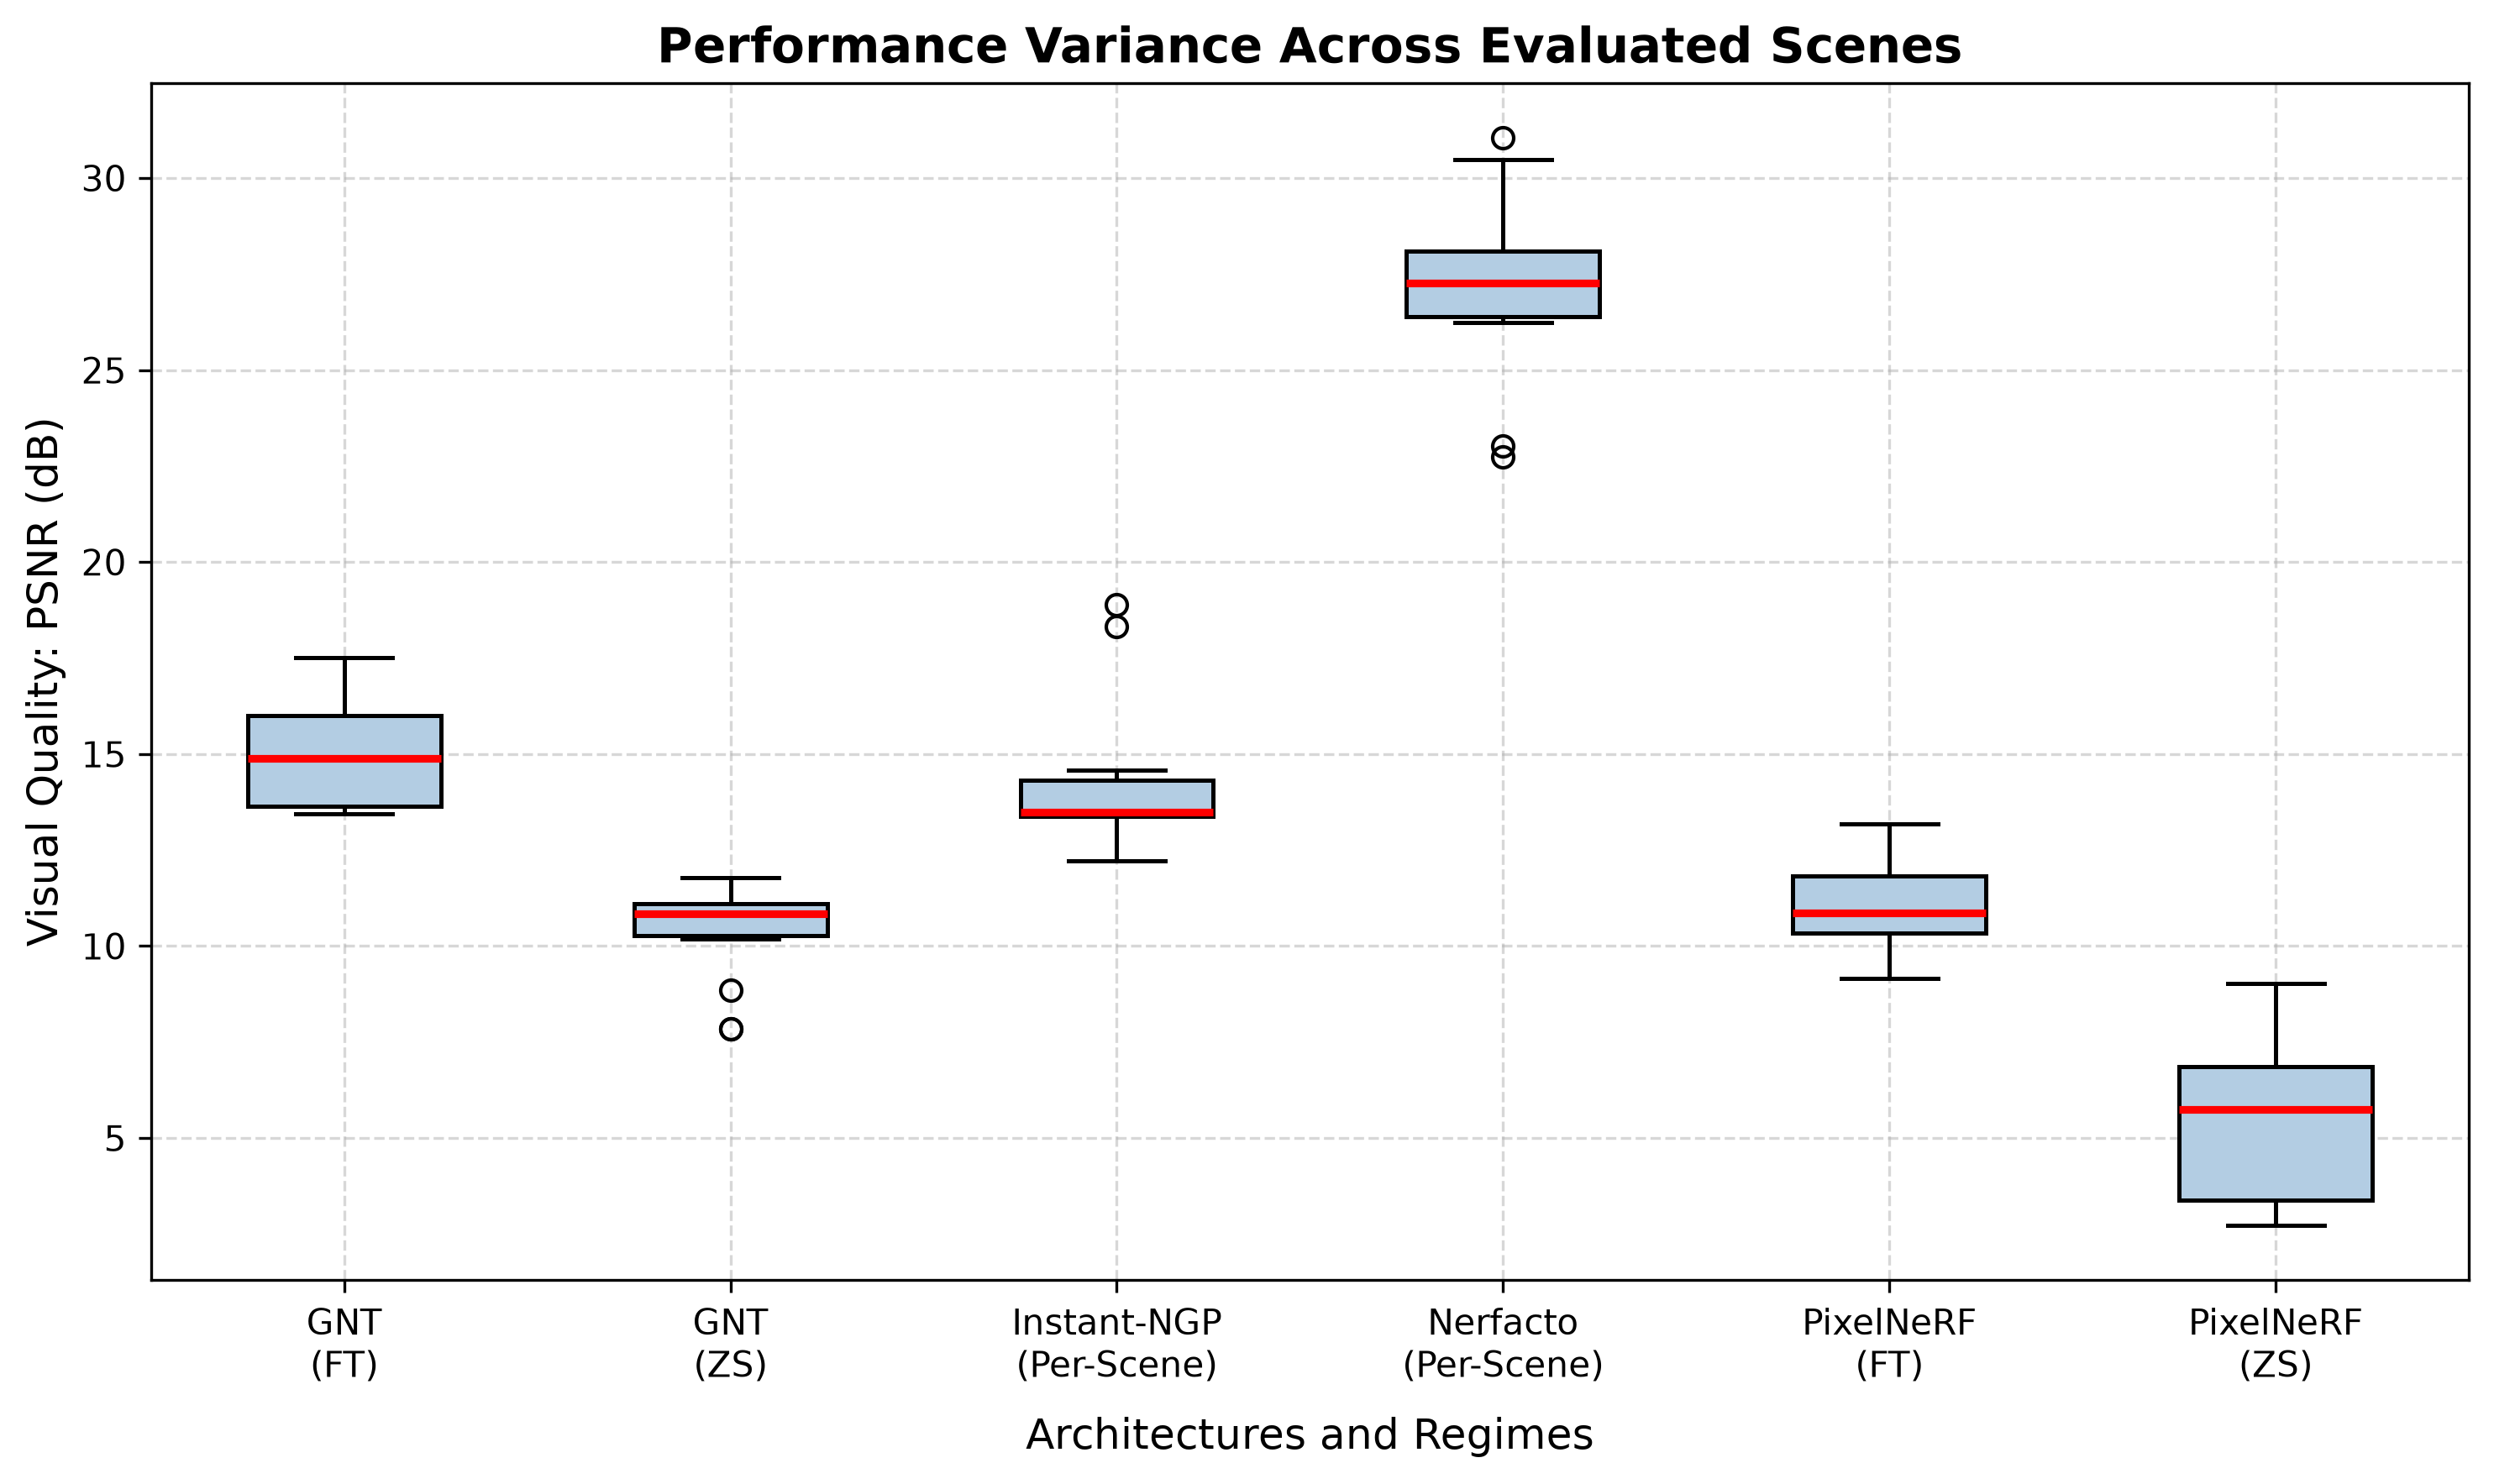
\includegraphics[width=0.84\linewidth]{img/plot_boxplot_fix.png}
\vspace{-3pt}
\caption{PSNR distributions across valid LLFF scenes ($N=10$ for per-scene baselines; optimal FT vs.\ ZS for generalizable models). Red horizontal lines indicate medians and boxes represent interquartile ranges (IQR). Fine-tuned GNT achieved a higher median PSNR than Instant-NGP ($15.07$ vs.\ $14.06$ dB), while Nerfacto reached the highest overall distribution ($27.11$ dB mean).}
\label{fig:boxplot}
\end{figure}

\begin{figure}[!t]
\centering
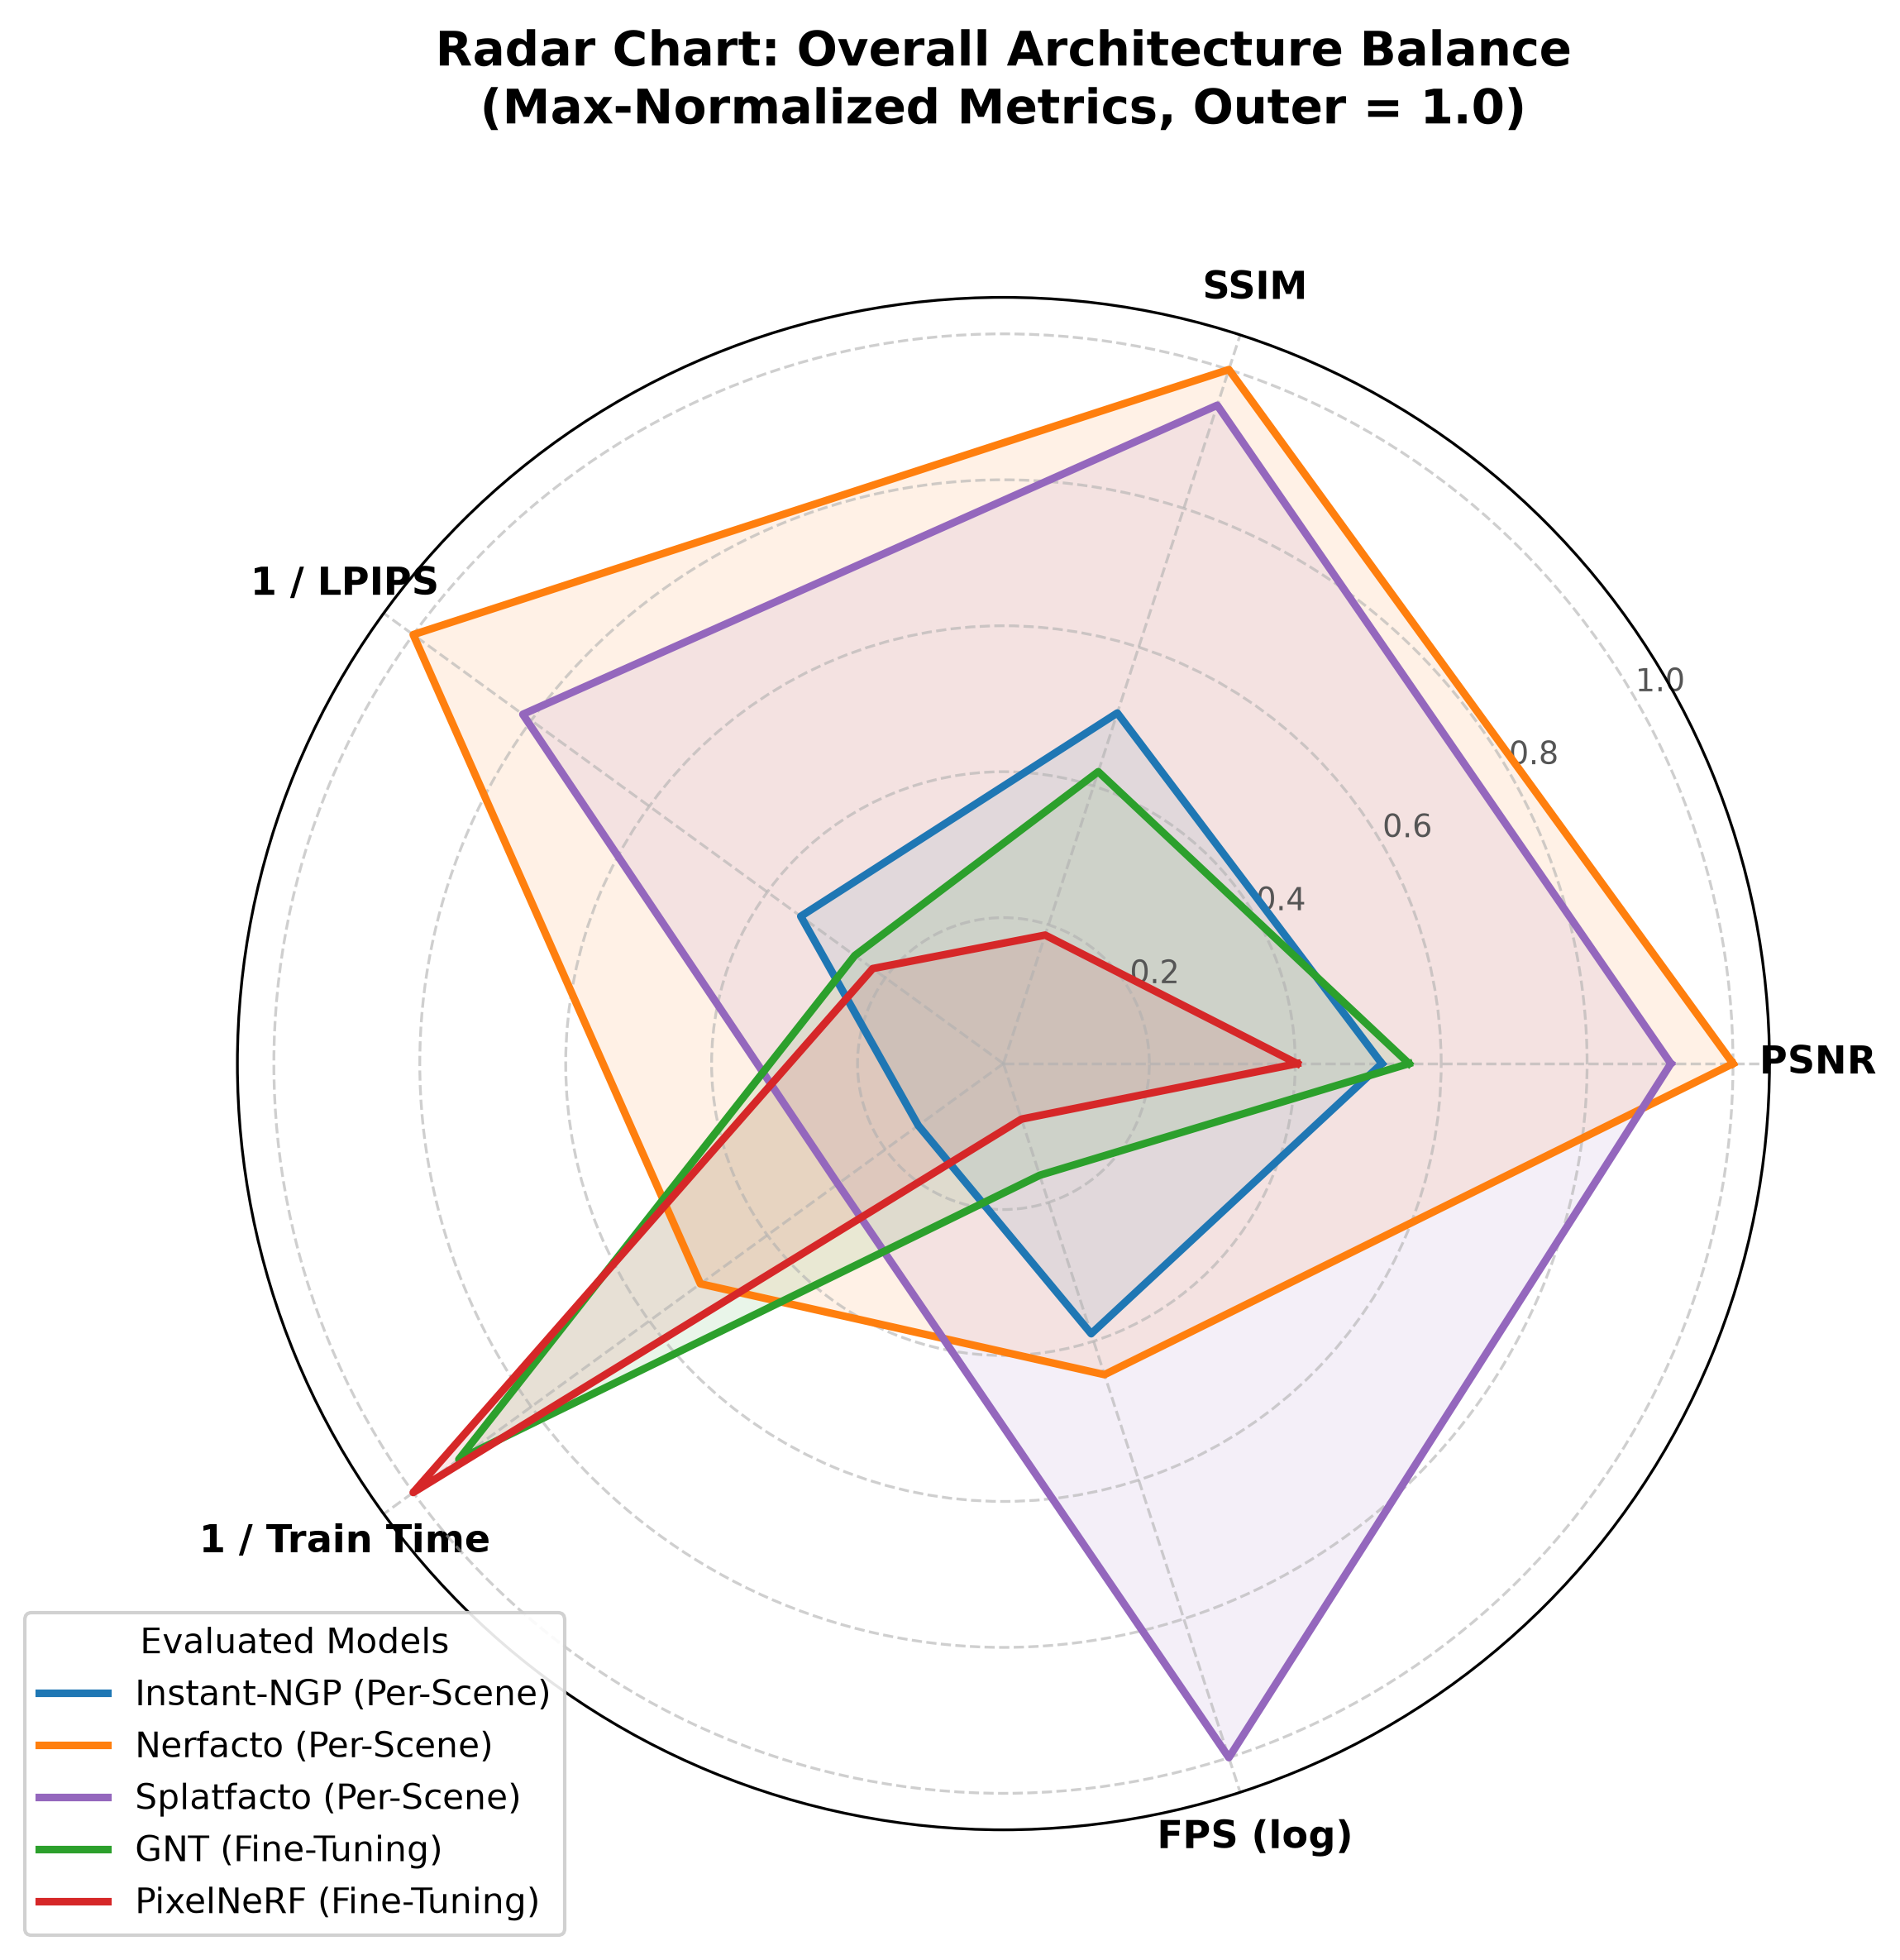
\includegraphics[width=0.74\linewidth]{img/plot_radar_fix.png}
\vspace{-3pt}
\caption{Multi-metric trade-offs under sparse-view conditions ($N=10$). Metrics were max-normalized to $[0,1]$ (outer perimeter = best), using $1/\text{LPIPS}$, $1/\text{Train Time}$, and log-scaled FPS. Splatfacto led in rendering speed ($200.7$ FPS) and Nerfacto led in visual fidelity, whereas fine-tuned GNT required the shortest adaptation time ($\sim 5\text{ min}$) but exhibited low rendering FPS.}
\label{fig:radar_chart}
\end{figure}

Comparing training time against inference throughput highlights the operational trade-off between both families of methods. Generalizable models required only $\sim 9\text{--}22\text{ s}$ for Zero-Shot evaluation or $\sim 4.6\text{--}5.0\text{ min}$ for 500-step fine-tuning, but projecting multi-view features and evaluating epipolar attention along each ray limited rendering throughput to $0.006$ FPS in PixelNeRF and $0.015$ FPS in GNT, with $\sim 1.94$ GB of dynamic VRAM. Per-scene hash-grid models increased inference speed to $0.199$ FPS in Instant-NGP and $0.388$ FPS in Nerfacto. Using explicit tile-based rasterization, Splatfacto (3DGS) reached $200.7$ FPS ($\approx 517\times$ faster than Nerfacto) while consuming $0.10$ GB of dynamic VRAM ($14.3\times$ less than Nerfacto's $1.43$ GB), requiring $16\text{ min }23\text{ s}$ of per-scene optimization. Consequently, PFT- and PEFT-adapted GNT was advantageous under extreme view scarcity ($N=3$) and short adaptation budgets, whereas Splatfacto and Nerfacto were superior when $N \ge 10$ views and longer training times were available.

\subsection{Qualitative Analysis}
Figure~\ref{fig:comparacao_qualitativa} shows novel views rendered across five LLFF scenes (\textit{Fern}, \textit{Flower}, \textit{Fortress}, \textit{Horns}, and \textit{Room}) under $N=10$ input views.

In Column 1, PixelNeRF adapted with \textit{PFT-Backbone} recovered the global color palette and coarse object contours in structured scenes such as \textit{Fortress} and \textit{Room}. However, because its coordinate MLP averages projected features without explicit depth reasoning, scenes with multi-layer occlusions (\textit{Fern} and \textit{Horns}) exhibited heavy spatial smoothing, consistent with its $0.772$ LPIPS score.

Columns 2 to 4 show the visual progression across the GNT fine-tuning strategies as the number of adapted parameters in the decoder increased. In Column 2, \textit{BitFit} ($<0.15\%$ trainable weights) corrected zero-shot color shifts and reduced near-camera floaters, but left fine surface textures blurred. In Column 3, adding rank-$4$ adapters via \textit{PEFT-LoRA} sharpened object boundaries, recovering petal edges in \textit{Flower} and bone contours in \textit{Horns}. In Column 4, updating the full rendering head under \textit{PFT-Decoder} produced the sharpest reconstructions among the generalizable models ($15.07$ dB PSNR and $0.679$ LPIPS), separating overlapping leaves in \textit{Fern} and stone reliefs in \textit{Fortress}.

In Column 5, \textit{Splatfacto} (3DGS) produced the sharpest textures and depth boundaries across all five scenes. The explicit 3D Gaussian primitives reconstructed fine foliage details in \textit{Fern} and \textit{Flower} as well as background structures in \textit{Horns} and \textit{Room} at $200.7$ FPS, showing only localized elongated Gaussian artifacts near image borders where camera overlap was lower.

\begin{figure}[!t]
\centering
\tiny
\setlength{\tabcolsep}{0pt}
\renewcommand{\arraystretch}{0.38}
\begin{tabular}{@{}c@{\hspace{2.2pt}}c@{\hspace{1.1pt}}c@{\hspace{1.1pt}}c@{\hspace{1.1pt}}c@{\hspace{1.1pt}}c@{}}
& \shortstack{\textbf{PixelNeRF}\\\tiny (Backbone)} & \shortstack{\textbf{GNT}\\\tiny (BitFit)} & \shortstack{\textbf{GNT}\\\tiny (LoRA)} & \shortstack{\textbf{GNT}\\\tiny (Decoder)} & \shortstack{\textbf{Splatfacto}\\\tiny (3DGS)} \\[1.8pt]
\raisebox{13pt}{\textbf{Fern}} &

\includegraphics[width=0.174\linewidth]{img/grid5x5/fern_pixelnerf_ft.png} &

\includegraphics[width=0.174\linewidth]{img/grid5x5/fern_gnt_bitfit.png} &
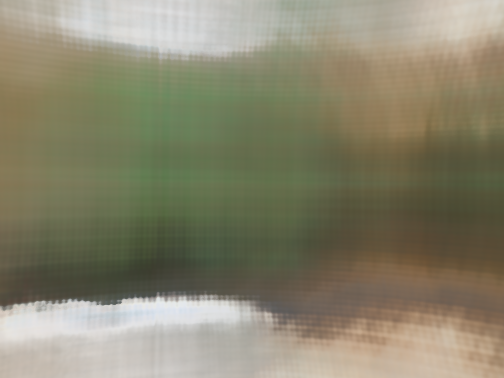
\includegraphics[width=0.174\linewidth]{img/grid5x5/fern_gnt_lora.png} &
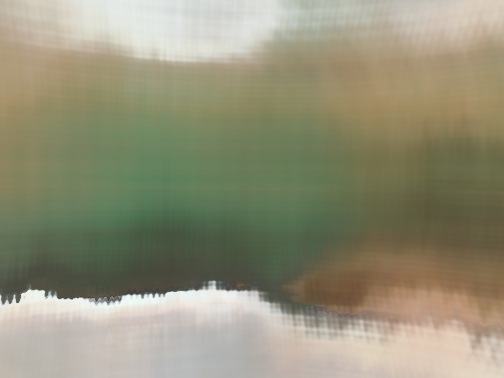
\includegraphics[width=0.174\linewidth]{img/grid5x5/fern_gnt_ft.png} &

\includegraphics[width=0.174\linewidth]{img/grid5x5/fern_splatfacto.png} \\[1.0pt]
\raisebox{13pt}{\textbf{Flower}} &

\includegraphics[width=0.174\linewidth]{img/grid5x5/flower_pixelnerf_ft.png} &

\includegraphics[width=0.174\linewidth]{img/grid5x5/flower_gnt_bitfit.png} &
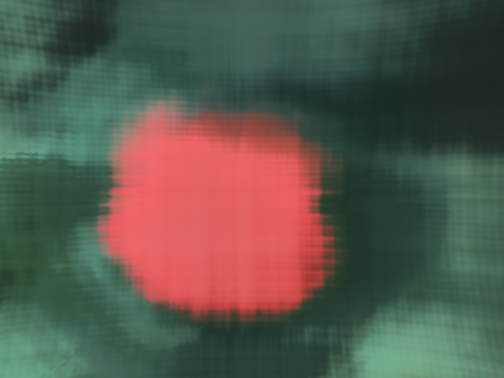
\includegraphics[width=0.174\linewidth]{img/grid5x5/flower_gnt_lora.png} &
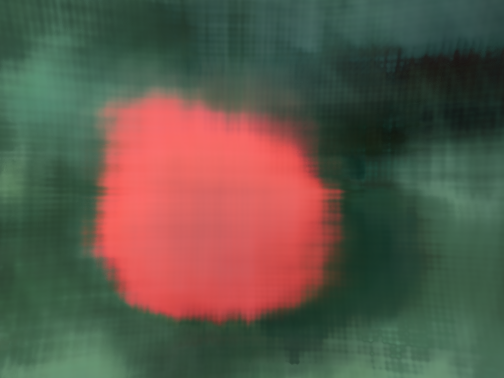
\includegraphics[width=0.174\linewidth]{img/grid5x5/flower_gnt_ft.png} &

\includegraphics[width=0.174\linewidth]{img/grid5x5/flower_splatfacto.png} \\[1.0pt]
\raisebox{13pt}{\textbf{Fortress}} &

\includegraphics[width=0.174\linewidth]{img/grid5x5/fortress_pixelnerf_ft.png} &
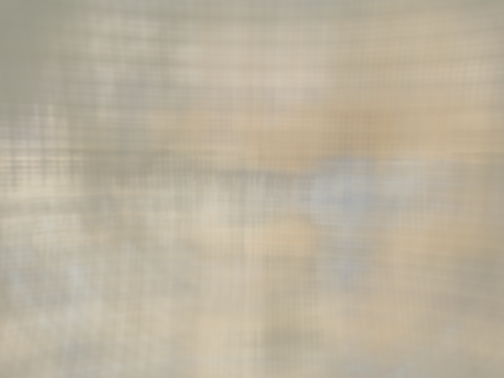
\includegraphics[width=0.174\linewidth]{img/grid5x5/fortress_gnt_bitfit.png} &
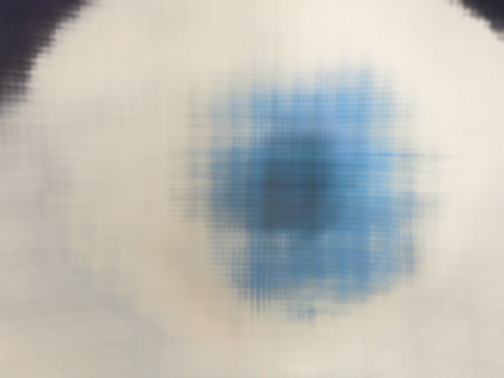
\includegraphics[width=0.174\linewidth]{img/grid5x5/fortress_gnt_lora.png} &
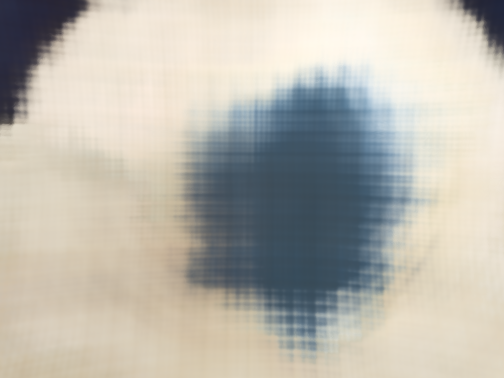
\includegraphics[width=0.174\linewidth]{img/grid5x5/fortress_gnt_ft.png} &
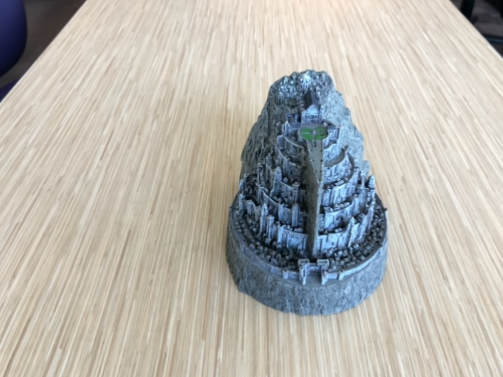
\includegraphics[width=0.174\linewidth]{img/grid5x5/fortress_splatfacto.png} \\[1.0pt]
\raisebox{13pt}{\textbf{Horns}} &

\includegraphics[width=0.174\linewidth]{img/grid5x5/horns_pixelnerf_ft.png} &

\includegraphics[width=0.174\linewidth]{img/grid5x5/horns_gnt_bitfit.png} &
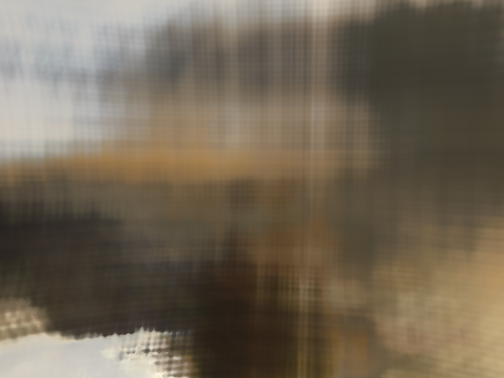
\includegraphics[width=0.174\linewidth]{img/grid5x5/horns_gnt_lora.png} &
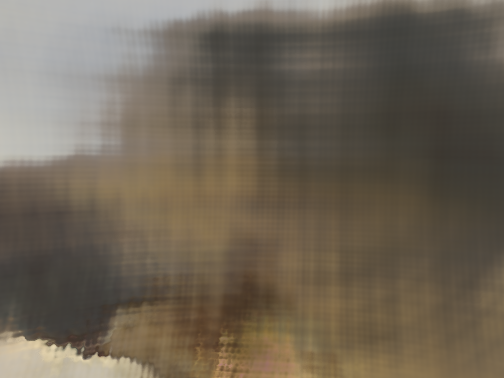
\includegraphics[width=0.174\linewidth]{img/grid5x5/horns_gnt_ft.png} &
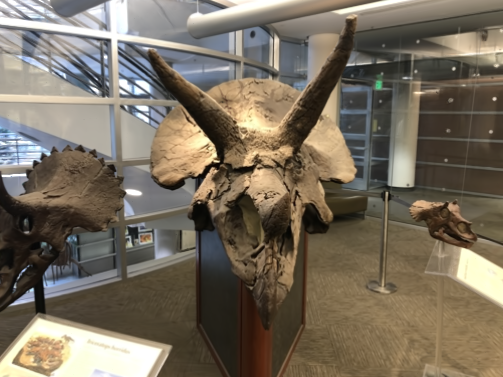
\includegraphics[width=0.174\linewidth]{img/grid5x5/horns_splatfacto.png} \\[1.0pt]
\raisebox{13pt}{\textbf{Room}} &

\includegraphics[width=0.174\linewidth]{img/grid5x5/room_pixelnerf_ft.png} &
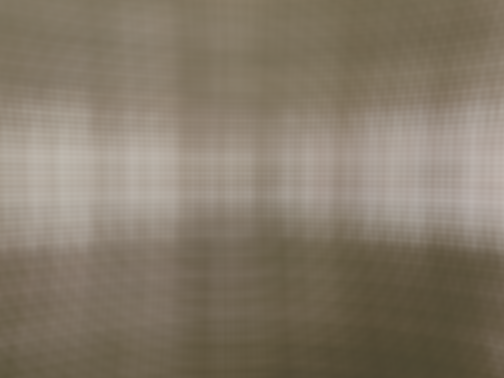
\includegraphics[width=0.174\linewidth]{img/grid5x5/room_gnt_bitfit.png} &
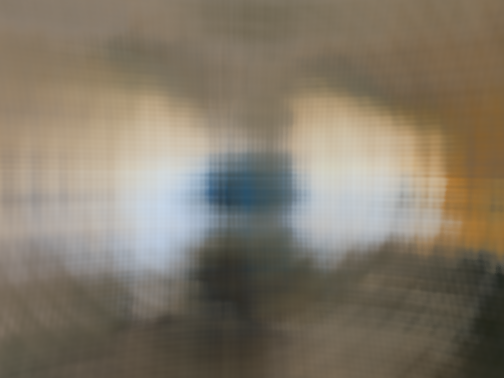
\includegraphics[width=0.174\linewidth]{img/grid5x5/room_gnt_lora.png} &
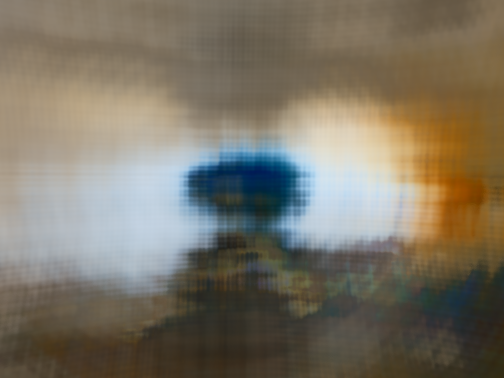
\includegraphics[width=0.174\linewidth]{img/grid5x5/room_gnt_ft.png} &

\includegraphics[width=0.174\linewidth]{img/grid5x5/room_splatfacto.png} \\
\end{tabular}
\vspace{-4pt}
\caption{Qualitative comparison across five LLFF scenes under $N=10$ input views. From left to right: PixelNeRF adapted with PFT-Backbone (Col.\ 1), GNT adapted with BitFit (Col.\ 2), PEFT-LoRA ($r=4$, Col.\ 3), and PFT-Decoder (Col.\ 4), and per-scene Splatfacto / 3DGS (Col.\ 5). Increasing the adapted parameter capacity in the GNT decoder progressively sharpened object contours, while Splatfacto preserved the finest high-frequency details at $>200$ FPS.}
\label{fig:comparacao_qualitativa}
\end{figure}
